%Jennifer Pan, August 2011

\documentclass[10pt,letter]{article}
	% basic article document class
	% use percent signs to make comments to yourself -- they will not show up.

\usepackage{amsmath}
\usepackage{amssymb}
	% packages that allow mathematical formatting

\usepackage{graphicx}
	% package that allows you to include graphics

\usepackage{enumitem}

\usepackage{setspace}
	% package that allows you to change spacing

\onehalfspacing
	% text become 1.5 spaced

\usepackage{bbm}
\usepackage{fullpage}
	% package that specifies normal margins

\renewcommand{\vector}[1]{\boldsymbol{#1}}
\newcommand{\problem}[1]{\section*{Problem #1}}
\newcommand{\problempart}[1]{\paragraph{#1}}

\begin{document}
	% line of code telling latex that your document is beginning


\title{Problem Set 5}

\author{Nicholas Wu}

\date{Fall 2020}
	% Note: when you omit this command, the current dateis automatically included

\maketitle
	% tells latex to follow your header (e.g., title, author) commands.
\textbf{Note:} I use bold symbols to denote vectors and nonbolded symbols to denote scalars. I primarily use vector notation to shorthand some of the sums, since many of the sums are dot products.

\problem{1}

\problempart{(1)}
Let $s_0 = (3, 1)$, and $s_1 = (1,3)$. Define the set $S = \{ s_0, s_1 \}$. Then a history is given by a sequence:
\[ s_t = \{ s_j \}_{i=1}^t \]
for $j \in \{ 0, 1 \}$. Specifically, the set of histories $S^t$ is given by
\[ S^t = S \times S^{t-1} \]
where $S^0 = S$. Then the probability
\[ \pi(s^t) = p^k (1-p)^{t - k} \]
where $k$ is the number of $s_0$'s in the sequence $s_t$.
\problempart{(2)} In the AD equilibrium, players trade the good at all time periods and states. An equilibrium thus consists of consumption sequences $ \{ \{ c^1(s^t), c^2(s^t) \}_{s^t} \}_{t=0}^\infty $, prices $\{ \{ p(s^t) \}_{s^t} \}_{t=0}^\infty$
such that
\begin{itemize}
\item Each consumer $i \in \{A, B \}$'s consumption solves the utility maximization at the prices:
\[ \max \sum_{t=0}^\infty \beta^t \sum_{s^t \in S^t} \pi(s^t) \log(c^i(s^t)) \]
subject to
\[ \sum_{t=0}^\infty \sum_{s^t \in S^t} p(s^t) c^i(s^t) \le \sum_{t=0}^\infty \sum_{s^t \in S^t} p(s^t) \omega^i(s^t) \]
\item Markets clear: for all $t, s^t$,
\[ c^A(s^t) + c^B(s^t) = 4 \]
\end{itemize}
\problempart{(3)}
Solving the FOC for the consumer, we have
\[ \beta^t\frac{\pi(s^t)}{c^i(s^t)} - \lambda p(s^t) = 0 \]
\[ \lambda = \beta^t\frac{\pi(s^t)}{p(s^t)c^i(s^t)} \]
At $t=0$, there is a fixed start state history, so we have
\[ \lambda = \frac{1}{c^i(s^0)} \]
Then we have
\[  c^i(s^t) = \beta^t \pi(s^t) \frac{c^i(s_0)}{p(s^t)} \]
Summing $i$ and using the market clearing condition, we get
\[  4 = \beta^t \pi(s^t) \frac{4}{p(s^t)} \]
\[ p(s^t) = \beta^t \pi(s^t) \]

\problempart{(4)}
Using the prices derived in the previous part, we get
\[ c^i(s^t) = c^i(s_0) \]
And hence consumption is constant over time. Now, note that since the endowment probability is independent of history:
\[ \sum_{s^t} p(s^t)\omega^A(s^t) = \sum_{s^t} \beta^t \pi(s^t) \omega^A(s^t) = \beta^t (p(3) + (1-p)1 ) \]
\[ = \beta^t (1 + 2p)\]
Likewise
\[ \sum_{s^t} p(s^t)\omega^B(s^t) = \sum_{s^t} \beta^t \pi(s^t) \omega^B(s^t) = \beta^t (p(1) + (1-p)(3) ) \]
\[ = \beta^t (3 - 2p)\]
Then from the budget constraint:
\[ \sum_{t=0}^\infty \sum_{s^t \in S^t} p(s^t) c^A(s^t) = \sum_{t=0}^\infty \sum_{s^t \in S^t} p(s^t) \omega^A(s^t) \]
\[ \sum_{t=0}^\infty \sum_{s^t \in S^t} \beta^t \pi(s^t) c^A(s^0) = 3 + \sum_{t=1}^\infty \beta^t (1 + 2p) \]
\[ c^A(s^0) \sum_{t=0}^\infty \beta^t \sum_{s^t \in S^t}  \pi(s^t)  = 3 + (1 + 2p) \sum_{t=1}^\infty \beta^t  \]
\[ \frac{ c^A(s^0)}{1-\beta} = 3 + \frac{\beta (1 + 2p)}{1-\beta} \]
\[ c^A(s^t) = c^A(s^0) = 3(1-\beta) + \beta(1+2p) = 3 - 2\beta (1-p) \]
and
\[ c^B(s^t) = 4 - c^A(s^t) = 1 + 2\beta (1-p) \]

\pagebreak
\problem{2}

\problempart{(1)}
We first define a history as an element $s^t \in S^t$, where $S^0 = \{ H, L\}$ and
\[ S^t = S^{t-1} \times \{ H, L \} \]
The probability of a given history is then
\[ \pi(s^t) = p \pi(s^{t-1}) \mathbbm{1}_{s^{t}_{t-1} = s^t_{t}} + (1-p) \pi(s^{t-1}) \mathbbm{1}_{s^{t}_{t-1} \neq s^t_{t}}\]
where $s^t_k$ denotes the state at time $k$ in history $s^t$, and $s^{t-1}$ denotes the truncation of history $s^t$ at time $t-1$, and we use $\mathbbm{1}_E$ as an indicator for event $E$.

Now, we can define an AD equilibrium. An AD equilibrium consists of consumption and capital savings sequences $ \{ \{ c(s^t), k(s^t) \}_{s^t} \}_{t=0}^\infty $, prices $\{ \{ p(s^t), w(s^t), r^k(s^t) \}_{s^t} \}_{t=0}^\infty$, firm allocations $\{ \{ l^f(s^t), k^f(s^t) \}_{s^t} \}_{t=0}^\infty $
such that
\begin{itemize}
\item Consumers maximize utility:
\[ \max_{c, k} \sum_{t=0}^\infty \beta^t \sum_{s^t} \pi(s^t) u(c(s^t)) \]
subject to
\[ \sum_{t=0}^\infty\sum_{s^t} p(s^t) (c(s^t) + k(s^t)) \le \sum_{t=0}^\infty\sum_{s^t} p(s^t)(w(s^t) + (1+r^k(s^t) - \delta) k(s^{t-1}))  \]
\[ k(s^{-1}) = \frac{\bar{k}}{1-\delta} \]
(dividing such that the initially available amount of consumption at the initial state is $\bar{k}$).
\item Firms maximize profit: $l^f, k^f$ satisfy:
\[ \max_{k, l} z(s^t) k^f(s^t)^{\alpha} l^f(s^t)^{1-\alpha} - r^k(s^t) k^f(s^t) - w(s^t)l(s^t) \]
\item Markets clear:
\[ k^f(s^t) = k(s,^t) \]
\[ l^f(s^t) = 1 \]
\[ c(s^t) + k(s^t) = z(s^t) k(s^{t-1})^\alpha + (1-\delta)k(s^{t-1}) \]
\end{itemize}
\problempart{(2)}
The social planner problem is to choose capital investment levels $k(s^t)$ such that
\[ \max \sum_{t=0}^\infty \beta^t \sum_{s^t} \pi(s^t) u(z(s^t)k(s^{t-1})^\alpha + (1-\delta)k(s^{t-1}) - k(s^t)) \]
We start with the AD equilibrium conditions. Taking the FOC of the firm's problem and applying market clearing, we get
\[ r^k(s^t) = \alpha z(s^t) k(s^t)^{\alpha - 1} \]
\[ w(s^t) = (1-\alpha)z(s^t)k(s^t)^\alpha \]
Now, we take the FOCs for the consumer problem.
\[ \beta^t \pi(s^t) u'(c(s^t)) = p(s^t) \]
For each state $s^t$, we can take the FOC for $k(s^t)$. Fix $z$ as the state at the end of $s^t$, and let $z' \neq z$. To clean up notation, let us also define $s^{t+1}_z$ as the history that ends with state $z$ after $s^t$, and $s^{t+1}_{z'}$ as the history ending with $z'$ after $s^t$.
\[ p(s^t) = p(s^{t+1}_z)(r^k(s^{t+1}_z) + 1 - \delta) + p(s^{t+1}_{z'})(r^k(s^{t+1}_{z'}) + 1 - \delta)  \]
Plugging in the other FOC, we get
\[ \beta^t \pi(s^t) u'(c(s^t)) = \beta^{t+1} \pi(s^{t+1}_z) u'(c(s^{t+1}_z))(r^k(s^{t+1}_z) + 1 - \delta) + \beta^{t+1} \pi(s^{t+1}_{z'}) u'(c(s^{t+1}_{z'})) (r^k(s^{t+1}_{z'}) + 1 - \delta) \]
Using the recursion on $\pi$, we get
\[ \frac{1}{\beta }u'(c(s^t)) = p u'(c(s^{t+1}_z))(\alpha z k(s^t)^{\alpha - 1} + 1 - \delta) + (1-p) u'(c(s^{t+1}_{z'})) (\alpha z' k(s^t)^{\alpha - 1}+ 1 - \delta) \]

Now we investigate the social planner problem. The FOCs for the social planner problem are:
\[ \beta^{t+1}\pi(s^{t+1}_{z})u'(z k(s^{t})^\alpha + (1-\delta)k(s^{t}) - k(s^{t+1}))(\alpha z k(s^t)^{\alpha - 1} + (1-\delta)) \] \[ + \beta^{t+1}\pi(s^{t+1}_{z'})u'(z' k(s^{t})^\alpha + (1-\delta)k(s^{t}) - k(s^{t+1}))(\alpha z' k(s^t)^{\alpha - 1} + (1-\delta)) \] \[  - \beta^t \pi(s^t) u'(z k(s^{t-1})^\alpha + (1-\delta)k(s^{t-1}) - k(s^t)) = 0 \]
Using the recursion on $\pi$, we can simplify this
\[ \beta pu'(z k(s^{t})^\alpha + (1-\delta)k(s^{t}) - k(s^{t+1}))(\alpha z k(s^t)^{\alpha - 1} + (1-\delta))   \]
\[ + \beta (1-p) u'(z' k(s^{t})^\alpha + (1-\delta)k(s^{t}) - k(s^{t+1}))(\alpha z' k(s^t)^{\alpha - 1} + (1-\delta)) \]
\[ =  u'(z k(s^{t-1})^\alpha + (1-\delta)k(s^{t-1}) - k(s^t)) \]
Substituting $c(s^t)$ for sake of cleanliness, we get
\[ \frac{u'(c(s^t))}{\beta} = pu'(c(s^{t+1}_z))(\alpha z k(s^t)^{\alpha - 1} + (1-\delta)) + (1-p)u'(c(s^{t+1}_{z'}))(\alpha z' k(s^t)^{\alpha - 1} + (1-\delta)) \]
This is exactly the same condition we found for the AD equilibrium. Hence the AD equilibrium allocation is efficient.
\problempart{(3)}
The value function needs to know the previous period capital investment and the current state.
\[ V(k, z) = \max_{k'} u(zk^{\alpha} + (1-\delta)k - k') + \beta p V(k', z) + \beta(1-p) V(k', z') \]
subject to
\[ 0 \le k' \le zk^{\alpha} + (1-\delta)k \]
where $z \neq z'$, $z, z' \in \{ z_H, z_L\}$.
\problempart{(4)} See separate code, and figure 1 for policy functions. We note that at $p=0.95$, the consumer believes that they will stay in their current state with higher probability, and hence they will save less in the high state and save more in the lower state than at $p=0.5$.
\begin{figure}
\centering
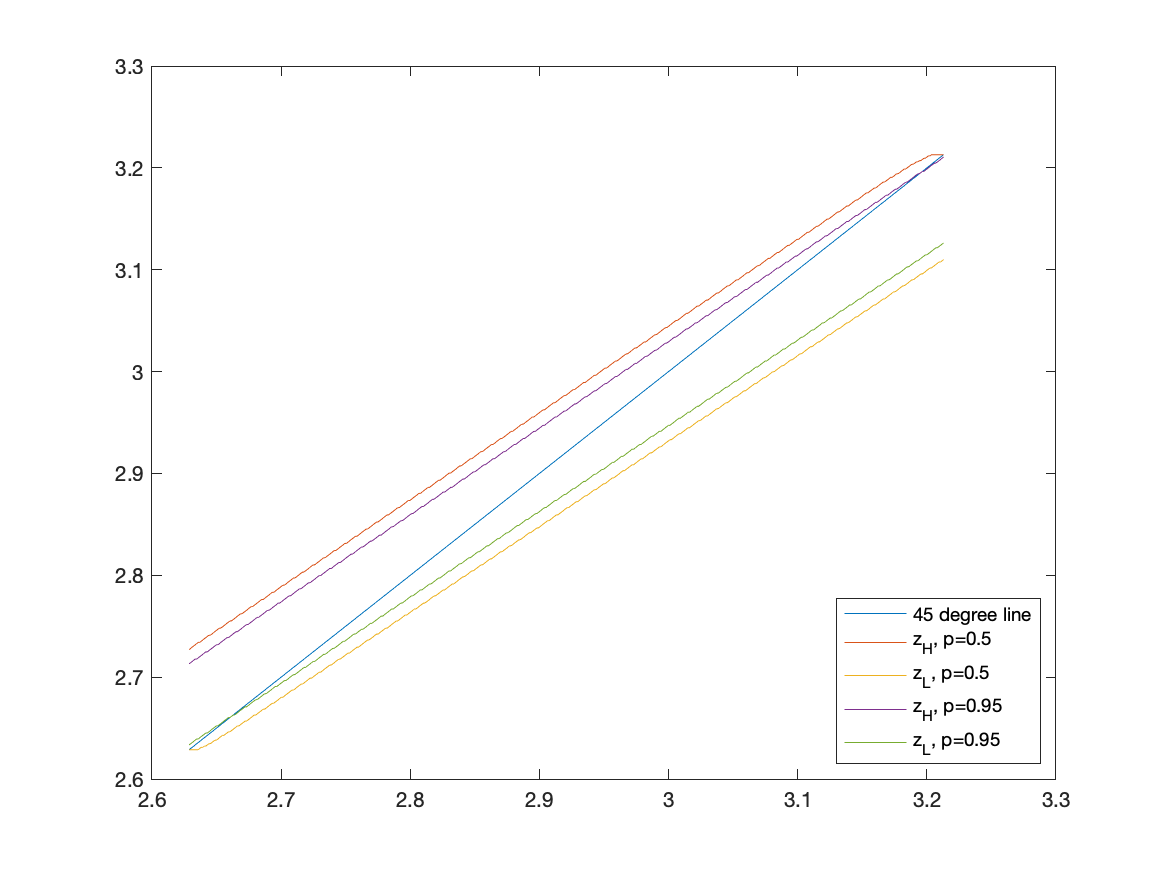
\includegraphics[scale=0.8]{ps5q2}
\caption{Question 2, part 4.}
\end{figure}

\pagebreak
\problem{3}

\problempart{(1)}
The value function needs to know the current state in the Markov chain:
\[ V(k, z) = \max_{k'} u(z + (1+r)k - k') + p \beta V(k', z) + (1-p) \beta V(k', z') \]
where
\[ k, k' \ge \underline{b} \]
and $z \neq z', z, z' \in \{ z^H, z^L \}$.
\problempart{(2)}
See attached code and figure 2. There isn't a lot of relative variation in the consumer's income, so in both states if net income is high, the consumer will not save very much and push down savings. The only cases where the policy function could cause savings to increase is when the savings are very low and the consumer is in the high income state.
\begin{figure}
\centering
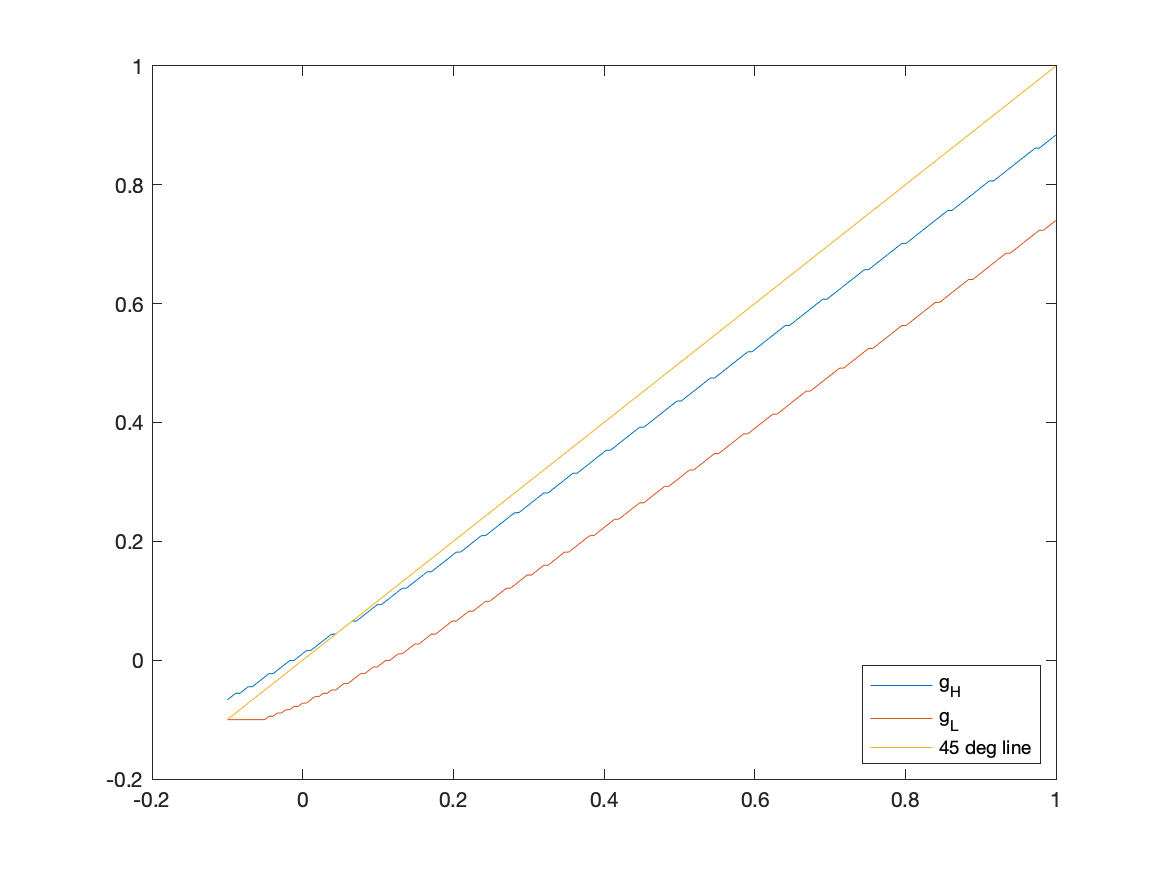
\includegraphics[scale=0.8]{ps5q3p2}
\caption{Question 3, part 2.}
\end{figure}
\problempart{(3)}
See attached code.

In figure 3, we vary $p$ between $0.5$ and $0.95$. We note that as $p \to 1$, the savings behavior in the high state decreases; as the consumer is more certain about staying with higher income, the consumer in the high state will not save as much than when the consumer is less certain. Similarly, in the low state, as $p \to 1$, the consumer is more certain about having lower income next period, and will thus save more than if the consumer thought there was a higher probability of transitioning to the higher state.

In figure 4, we vary $\epsilon$, from $0.1$ to $0.3$. We note that at higher $\epsilon$, the difference in income between the two states is more pronounced, and hence the more the savings behavior will compensate for the potential change in state; when the state is high and $\epsilon$ is higher, the lower state is worse, and the consumer saves more. When $\epsilon$ is high and the state is low, the consumer saves less than if $\epsilon$ was lower.

In figure 5, we vary $\underline{b}$, lowering from $-0.1$ to $-0.2$. We see that in both states, savings decreases at all levels. Since the consumer is less worried about hitting the borrowing constraint, the consumer generally saves less in either state.
\begin{figure}
\centering
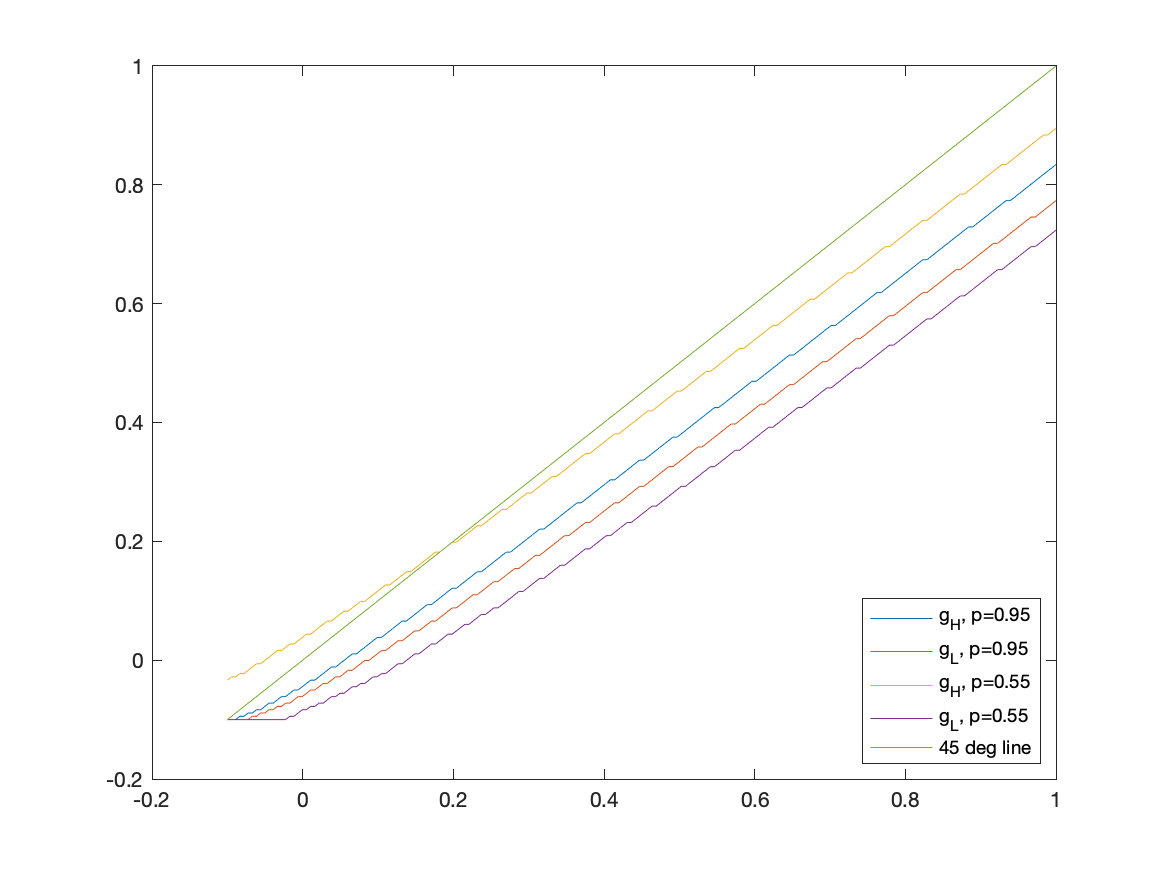
\includegraphics[scale=0.8]{ps5q3p3_1}
\caption{Question 3, part 3. Variation in $p$.}
\end{figure}
\begin{figure}
\centering
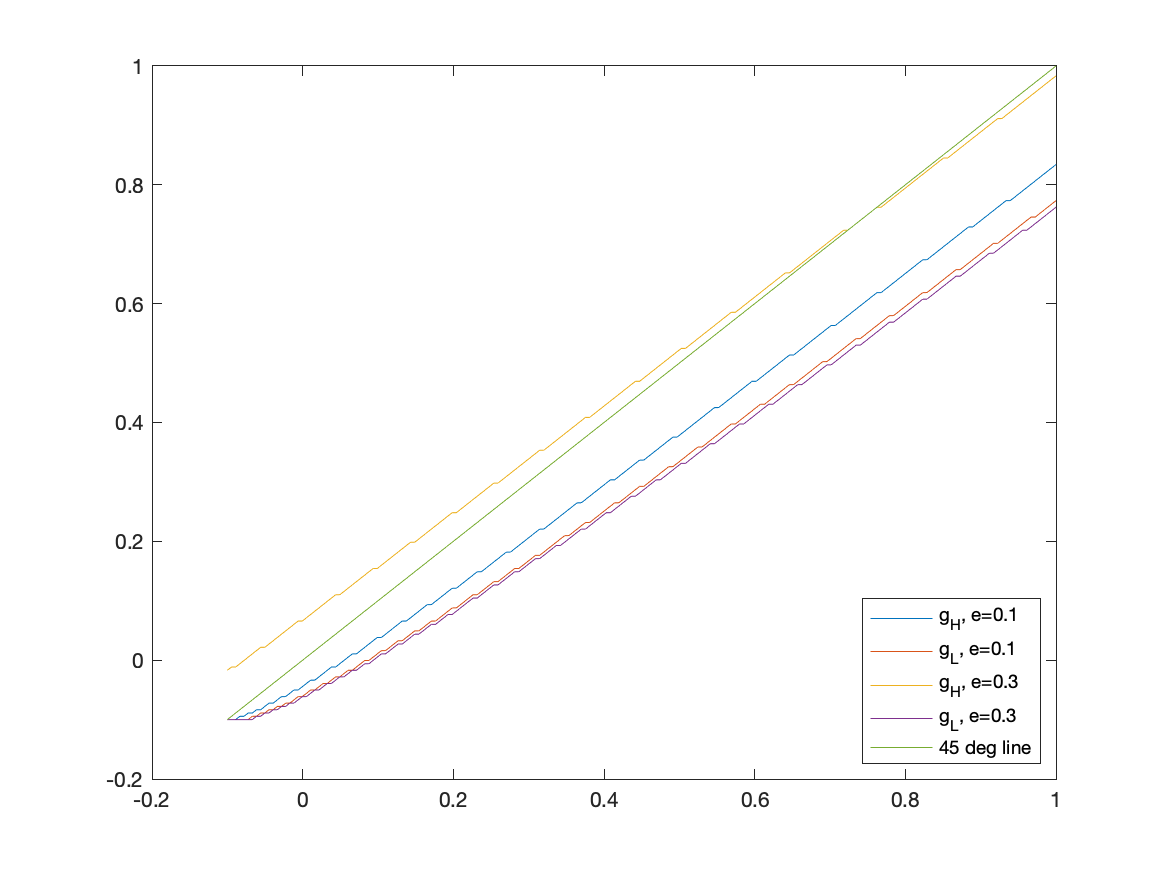
\includegraphics[scale=0.8]{ps5q3p3_2}
\caption{Question 3, part 3. Variation in $\epsilon$.}
\end{figure}
\begin{figure}
\centering
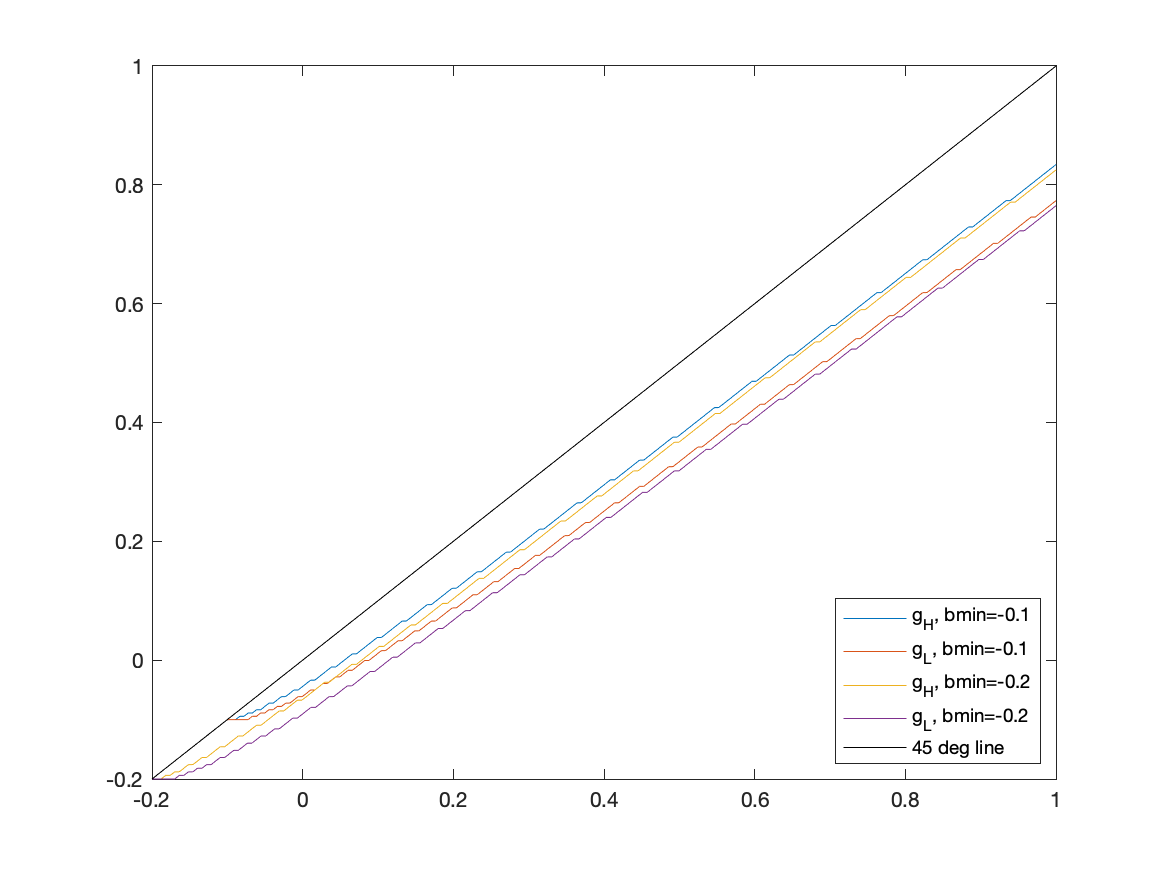
\includegraphics[scale=0.8]{ps5q3p3_3}
\caption{Question 3, part 3. Variation in $\underline{b}$.}
\end{figure}
\end{document}
	% line of code telling latex that your document is ending. If you leave this out, you'll get an error
